% Drawing 80/03-4 -- folder 80, batch 03, archive page 51 (PDF page 52).
% Transcription: figure, à gauche : six droites, les côtés du triangle $a$, $b$, $c$ et trois droites $D_a$, $D_b$, $D_c$ issues des sommets ; points marqués $a$, $b$, $c$, $a'$, $b'$, $c'$ à l'intérieur, $\alpha$, $\beta$, $\gamma$ sur les côtés. « $9$ » est écrit en marge devant « sommets ». Au-dessus de « répartissent », un indice \uncertain{$D_{J'}$} ; au-dessus de « la configuration est » biffé, « correspondant », \uncertain{lu}
% Kind: triangle with three lines from the vertices. Method 2 (schematic redraw from the facsimile). Status: ok.
% Notes: Six lines: the sides of the triangle with vertices a, b, c and the lines D_a, D_b, D_c through them; the points a', b', c' inside, alpha, beta, gamma on the sides (gamma looks like a small x). Labels as read on the crop.
% Coordinates: 1 unit = 1 mm = 1/100 of the crop width (bbox in page fractions: [0.08, 0.5, 0.38, 0.7]).
% Redrawn by Claude (claude-opus-5-5), issue #73, 2026-11-07; not checked by a human; not compiled (no TeX in the session).
% Revised 2026-11-07 after Michel's check: labels enlarged.
% Rights: reproduces part of the work -- behind RENDER_TRANSCRIPTS, never published by itself.
\documentclass[tikz,border=3pt]{standalone}
\usepackage{amsmath,amssymb}
\usetikzlibrary{patterns,arrows.meta}
\tikzset{pencil/.style={black!45}, struck/.style={black!35}, mark/.style={circle,draw,inner sep=1.3pt}, pt/.style={circle,fill,inner sep=0.9pt}, opt/.style={circle,draw,fill=white,inner sep=1.1pt}}
\begin{document}
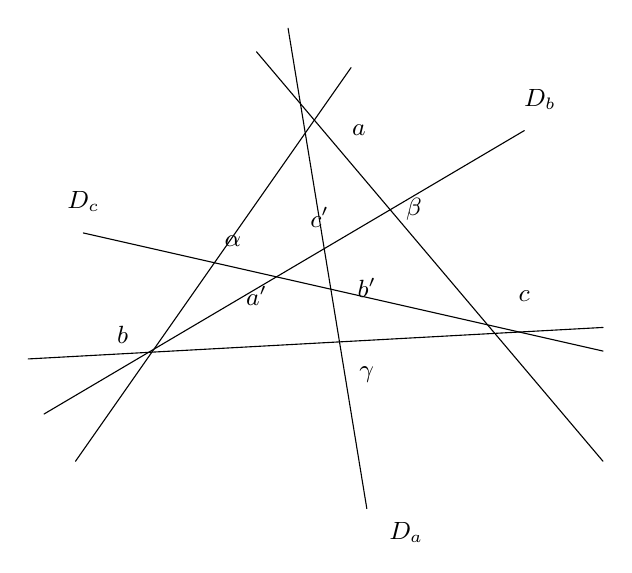
\begin{tikzpicture}[x=1mm,y=1mm,line cap=round,line join=round,font=\scriptsize]
\draw (60,-12) -- (70,-73);
\draw (68,-17) -- (33,-67);
\draw (56,-15) -- (100,-67);
\draw (27,-54) -- (100,-50);
\draw (34,-38) -- (100,-53);
\draw (29,-61) -- (90,-25);
\node[inner sep=1pt] at (69,-25) {\small $a$};
\node[inner sep=1pt] at (39,-51) {\small $b$};
\node[inner sep=1pt] at (90,-46) {\small $c$};
\node[inner sep=1pt] at (56,-46) {\small $a'$};
\node[inner sep=1pt] at (70,-45) {\small $b'$};
\node[inner sep=1pt] at (64,-36) {\small $c'$};
\node[inner sep=1pt] at (53,-39) {\small $\alpha$};
\node[inner sep=1pt] at (76,-35) {\small $\beta$};
\node[inner sep=1pt] at (70,-56) {\small $\gamma$};
\node[inner sep=1pt] at (75,-76) {\small $D_a$};
\node[inner sep=1pt] at (92,-21) {\small $D_b$};
\node[inner sep=1pt] at (34,-34) {\small $D_c$};
\end{tikzpicture}
\end{document}
